%%%  Template to prepare a defense of Bc./Mgr./... thesis
%%%  to be presented at MFF
%%%  (unofficial)
%%%
%%%  AUTHOR:  Arnošt Komárek
%%%           Department of Probability and Mathematical Statistics
%%%           Faculty of Mathematics and Physics, Charles University in Prague
%%%
%%%  LOG:    20150505  created by modification of some previous personal presentations
%%%          20170522  update related to new MFF logo
%%%  
%%%  ===========================================================================
\documentclass[c, 10pt]{beamer}


%%%%% Package needed if some accented letters in the presentation
%%%%% -------------------------------------------------------------
\usepackage[utf8]{inputenc}



\usepackage{pgf,tikz,pgfplots}
\pgfplotsset{compat=1.15}
\usepackage{mathrsfs}
\usetikzlibrary{arrows}
\usepackage{enumerate}





%%%%% Most beamer settings and other LaTeX commands
%%%%% are provided in the file below
%%%%% -----------------------------------------------------
%%%
%%%  Style for MFF related presentations
%%%  (unofficial)
%%%
%%%  AUTHOR:  Arnošt Komárek
%%%           Department of Probability and Mathematical Statistics
%%%           Faculty of Mathematics and Physics, Charles University in Prague
%%%
%%%  LOG:    20150430  created by modification of some previous personal presentations
%%%          20170522  modified (new MFF logo)
%%%  
%%%  ===========================================================================

%%%%% If to determine whether Czech or English version
%%%%% of a presentation is to be produced
%%%%% default = Czech
%%%%% ------------------------------------------------------
\newif\ifCZversion
\CZversiontrue

\ifCZversion\else\renewcommand{\uv}[1]{``#1''}\fi


%%%%% Included packages
%%%%% ----------------------------------------------------------
\usepackage{helvet}                       % font
\usepackage{amsmath, amssymb}
\usepackage{delarray}
\usepackage{multicol}
\usepackage{graphicx, fancybox}
\usepackage{psfrag}
\usepackage{fancyvrb}
\usepackage{eurosym}
\usepackage{bbding}
%\usepackage{marvosym}
\usepackage{wasysym}
\usepackage[czech]{babel}
\usepackage{mathrsfs}
\usepackage[pdftex]{bookmark}

\usepackage{bbm}	% For lowercase blackboard bold
\usepackage{multicol}  	% ultiple columns
\usepackage{enumerate}

%%%%% Some LaTeX commands
%%%%% ----------------------------------------------------------
\renewcommand{\arraystretch}{1.2}


%%%%% Some colors and related commands
%%%%% ----------------------------------------------------------

  %% Pantone 186 = "official" red of MFF
\definecolor{redmff}{rgb}{0.7892720,0.0651341,0.1455939}          

  %% First level color = black
\definecolor{colOne}{rgb}{0,0,0}
\newcommand{\tOne}[1]{\textcolor{colOne}{#1}}
\newcommand{\tOneb}[1]{\textcolor{colOne}{\textbf{#1}}}
\newcommand{\tOnei}[1]{\textcolor{colOne}{\textit{#1}}}

  %% Second level color = quite dark blue
\definecolor{colTwo}{rgb}{0,0,0.3}                
\newcommand{\tTwo}[1]{\textcolor{colTwo}{#1}}
\newcommand{\tTwob}[1]{\textcolor{colTwo}{\textbf{#1}}}
\newcommand{\tTwoi}[1]{\textcolor{colTwo}{\textit{#1}}}

  %% Third level color = something between blue3 and blue4
\definecolor{colThree}{rgb}{0,0,0.7}              
\newcommand{\tThree}[1]{\textcolor{colThree}{#1}}
\newcommand{\tThreeb}[1]{\textcolor{colThree}{\textbf{#1}}}
\newcommand{\tThreei}[1]{\textcolor{colThree}{\textit{#1}}}

  %% Color to alert (highlight) = MFF red
\definecolor{alertCol}{rgb}{0.7892720,0.0651341,0.1455939}
\newcommand{\tal}[1]{\alert{#1}}
\newcommand{\talb}[1]{\textbf{\alert{#1}}}
\newcommand{\tali}[1]{\textit{\alert{#1}}}

  %% White
\newcommand{\tw}[1]{\textcolor{white}{#1}}
\newcommand{\twb}[1]{\textcolor{white}{\textbf{#1}}}
\newcommand{\twi}[1]{\textcolor{white}{\textit{#1}}}

  %% Some other colors used somewhere
\definecolor{semiwhite}{gray}{0.98}
\definecolor{mffgray}{gray}{0.95}
\definecolor{semiblack}{gray}{0.5}
\definecolor{rred}{rgb}{0.5,0,0}


%%%%% Beamer stuff
%%%%% ----------------------------------------------------------
\mode<presentation> {

    %%% General theme of a presentation (some pre-specified themes)
    %%% ------------------------------------------------------------------
    %\usetheme{CambridgeUS}
    \usetheme{Warsaw}

    %%% Color schemes that will be used unless redefined below
    %%% ------------------------------------------------------------------
    %\usecolortheme{wolverine}
    \usecolortheme{beaver}


    %%% Color schemes for different elements of a presentation
    %%% ---------------------------------------------------------

      %%% Uncomment the two rows below if some background file (layout) is to be used
      %%% on all slides
    %\usebackgroundtemplate{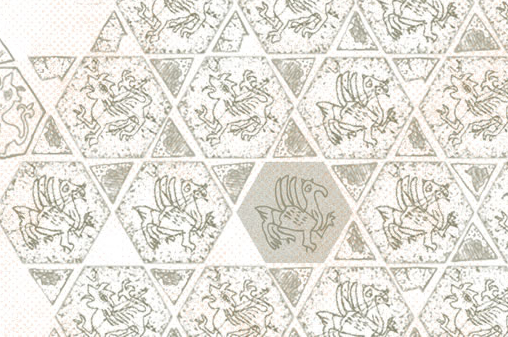
\includegraphics[width=\paperwidth, height=\paperheight]{./FigureLayout/BackgroundRotunda}}
    %\setbeamercolor{background canvas}{bg=}                                                             

      %%% Setting for "standard" slides
      %%% - must be commented if background file used
    \setbeamertemplate{background canvas}[vertical shading][bottom=semiwhite, top=white, middle=semiwhite!50!white]
    \setbeamercolor{background canvas}{bg=white}                           %% NO EFFECT WHEN \setbeamertemplate{background canvas} WAS USED

      %%% Colors of frametitle, normal, alerted and math texts
    \setbeamercolor{frametitle}{fg=white, bg=redmff}
    \setbeamercolor{normal text}{fg=black}
    \setbeamercolor{alerted text}{fg=redmff}
    \setbeamercolor{math text inlined}{fg=colTwo}
    \setbeamercolor{math text displayed}{fg=colTwo}

      %%% Colors for some special boxes defined below
    \setbeamercolor{mffboxcol}{fg=colTwo, bg=mffgray}
    \setbeamercolor{mffboxcolupper}{fg=white, bg=redmff}

    %%% Set serif font (patkové písmo) in mathematics
    %%% ------------------------------------------------
    %\usefonttheme[onlymath]{serif}

    %%% Itemize style (rectangles instead of bullets)
    %%% ------------------------------------------------
    % \useinnertheme{rectangles}

    %%% Default content of a header of each slide
    %%% (currently nothing)
    %%% ------------------------------------------------
    \setbeamertemplate{headline}{}

    %%% Default content of a foot of each slide
    %%% ------------------------------------------------
    %\setbeamercolor{page number in head/foot}{fg=black, bg=white}
    \setbeamertemplate{footline}{
      \hspace*{2.5em}
      \begin{beamercolorbox}{section in head/foot}
      \vskip1pt
      \tOne{\rule{\textwidth}{1pt}}
      \vskip2pt

      %%% Foot containing (a) page number/total number of pages, (b) name, (c) short title of presentation
      {\small \tOne{\insertframenumber}\textcolor{semiblack}{/\inserttotalframenumber}}\hspace{1em}
      \tOne{\footnotesize \insertauthor}\hfill
      \textcolor{redmff}{\footnotesize\insertshorttitle\hspace{3em}}

      %%% Foot containing (a) page number/total number of pages, (b) name, (c) short section title
      %{\small \tOne{\insertframenumber}\textcolor{semiblack}{/\inserttotalframenumber}}\hspace{1em}
      %\tOne{\footnotesize \insertauthor}\hfill
      %\textcolor{redmff}{\footnotesize\thesection. \insertsection\hspace{3em}}
    
      \hspace*{3.5em}
      \vskip3pt
      \end{beamercolorbox}
    }

    %%% Title page
    %%% -------------------
    \setbeamertemplate{title page}{
      %\vspace*{-0.5em}
      \begin{center}
      \textcolor{black}{\normalsize\bfseries\rmfamily \insertinstitute}

      \vspace{1em}
        
      \ifCZversion
        
\includegraphics[width=0.8\textwidth]{./FigureLayout/mff_cz_color}
      \else
        
\includegraphics[width=0.8\textwidth]{./FigureLayout/mff_en_color}
      \fi

      \medskip
      \noindent\textcolor{redmff}{\rule{\textwidth}{2pt}}
  
      \bigskip
      \textcolor{black}{\normalsize\bfseries \insertauthor} \\[0.5ex]

      \bigskip
      \textcolor{redmff}{\Large\bfseries \inserttitle}

      \medskip
      \textcolor{redmff}{\large\insertsubtitle}

      \medskip
      \noindent\textcolor{redmff}{\rule{\textwidth}{2pt}}
      
      \medskip
      \textcolor{colTwo}{\small \insertdate}
      \end{center}
    }    

    %%% Switch-off/on foot with navigation symbols    
    %%% -----------------------------------------------
    % \setbeamertemplate{navigation symbols}{}
    \usenavigationsymbolstemplate{}

    %%% Left and right margin
    %%% --------------------------------
    %\setbeamersize{text margin left=1cm}
    %\setbeamersize{text margin right=1cm}


    %%% Use of a logo on each slide
    %%% (not really recommended, so commented)
    %\logo{
\includegraphics[height=1.5cm, width=1.5cm]{./FigureLayout/mff_logo}}
}


%%%%% Commands to produce slides at the beginning of each section
%%%%% --------------------------------------------------------------
\renewcommand{\thesection}{\arabic{section}}
\newcommand{\framesection}{
  \begin{frame}%[plain]

  \vspace*{2em}
  \begin{center}\Large
  \ifCZversion Oddíl \thesection \else Section \thesection \fi
  \end{center}

  \begin{center}\color{rred}\Large
  \insertsection
  \end{center}

  \end{frame}
}


%%%%% Style for software related stuff
%%%%% ----------------------------------------------------------
\newcommand{\Rko}{
\includegraphics[width=5.094mm, height=3.876mm]{./FigureLayout/Rlogo}}
\newcommand{\Rfun}[1]{\textcolor{redmff}{\texttt{#1}}}

\DefineVerbatimEnvironment{Rin}{Verbatim}{formatcom=\color{redmff}, fontsize=\scriptsize, frame=single, framerule=1pt, framesep=2pt}
\DefineVerbatimEnvironment{Rout}{Verbatim}{formatcom=\color{blue}, fontsize=\scriptsize, frame=single, framerule=1pt, framesep=2pt}


%%%%% Boxes
%%%%% ----------------------------------------------------------
\newcommand{\mffbox}[2][0pt]{%
  \begin{beamercolorbox}[center, sep=#1, rounded=true, shadow=true]{mffboxcol}
  #2
  \end{beamercolorbox}
}

\newcommand{\mffboxTitle}[2]{%
  \begin{beamerboxesrounded}[lower=mffboxcol, upper=mffboxcolupper, shadow=true]{#1}
  #2
  \end{beamerboxesrounded}
}


%%%%% Some constructions for displayed math
%%%%% ----------------------------------------------------------
\newcommand{\dmath}[2][-1.4em]{%
  \begin{beamercolorbox}[center, sep=#1, rounded=true, shadow=true]{mffboxcol}
  \begin{displaymath}
  #2
  \end{displaymath}
  \end{beamercolorbox}
}

\newcommand{\dalign}[2][-1.4em]{%
  \begin{beamercolorbox}[center, sep=#1, rounded=true, shadow=true]{mffboxcol}
  \begin{align*}
  #2
  \end{align*}
  \end{beamercolorbox}
}

\newcommand{\dgather}[2][-1.4em]{%
  \begin{beamercolorbox}[center, sep=#1, rounded=true, shadow=true]{mffboxcol}
  \begin{gather*}
  #2
  \end{gather*}
  \end{beamercolorbox}
}



%%%%% \ifCZversion is defined inside MFF_Present.sty
%%%%% to distinguish between Czech and English presentations
%%%%% ------------------------------------------------------
%\CZversiontrue       %% for presentations in Czech (Slovak)
\CZversionfalse      %% for presentations in English


%%%%% Uncomment appropriate choice below if you wish to create
%%%%% notes for audience having 2 or 4 slides on each (A4) page.
%%%%% -------------------------------------------------------------
\usepackage{pgfpages}
%\pgfpagesuselayout{4 on 1}[a4paper, landscape, border shrink=5mm]
%\pgfpagesuselayout{2 on 1}[a4paper, border shrink=5mm]


%%%%% Basic settings of the document
%%%%% (will be automatically used to create a title page, foots etc.)
%%%%% --------------------------------------------------------------------

  %%% Main title
  %%% - short and long version
  %%%   --> will appear on place where \inserttitle and \insertshorttitle commands used
  %%%   --> if the full title is short enough, both short and long versions might be the same

\title[Generalized random tessellations]{%                       
	Generalized random tessellations, their properties, simulation and applications}

  %%% Subtitle (comment it if you do not want to have it)
  %%%   --> will appear on place where \insertsubtitle and \insertshortsubtitle commands used
 \subtitle[]{Thesis defense}

  %%% Author
  %%% - as "short" version, link to the author's webpage is used
  %%%   (e.g., e-mail is also a useful alternative)
  %%%   --> will appear on places where \insertauthor and \insertshortauthor commands used
\author[jahn@karlin.mff.cuni.cz]{%
        Daniel Jahn}

  %%% Author's affiliation
  %%% - can be fully commented for defense presentation
  %%%   --> will appear on places where \insertinstitute and \insertshortinstitute commands used
\institute[KPMS]{%
           Department of Probability and Mathematical Statistics}

  %%% Date of presentation
  %%% - replace it by real date in case of a defense presentation
  %%%   --> will appear on places where \insertdate and \insertshortdate commands used
\date[5.2.2019]{%
      5 February 2019}

      \newcommand{\x}{{\mathbbm{x}}}

\begin{document}


\setbeamertemplate{caption}{\insertcaption\par}

%%%%% Title slide
%%%%% =====================================================================================
\frame[noframenumbering,plain]{\titlepage}


% \begin{frame}\frametitle{Point and empty sphere property}\framesubtitle{Geometrical interpretation}p
% 
% 
% \begin{centering}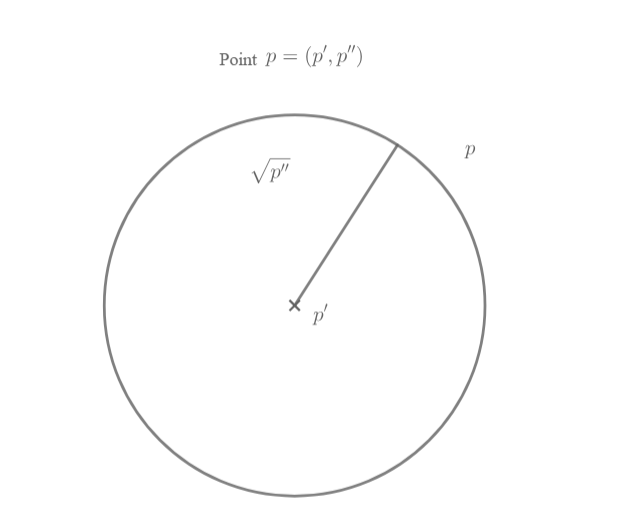
\includegraphics[height = 4.2cm]{./FigureLayout/point.PNG}
% 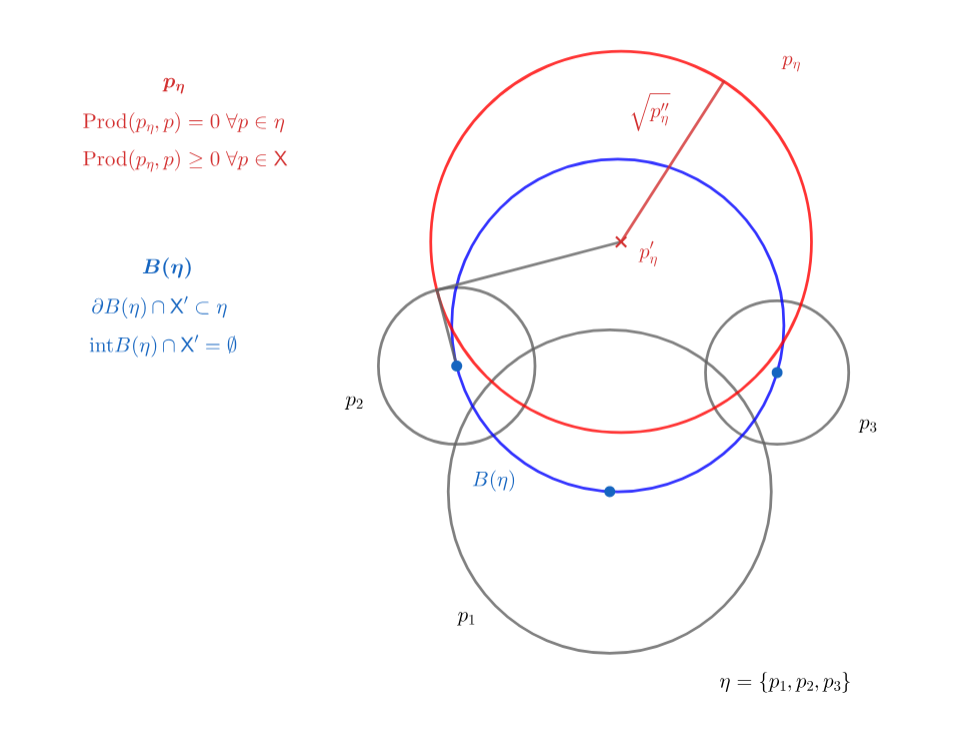
\includegraphics[height = 4.2cm]{./FigureLayout/power.PNG}\end{centering}
% \vspace{3mm}
% 
% where for $p,q \in \mathbb R^3 \times S$
% $$\text{Prod}(p,q) = \|p'-q'\|^2 - p'' - q''.$$
% 
% \end{frame}



\begin{frame}\frametitle{Delaunay tetrahedrization}
	Let $\x$ be a locally finite subset $\mathbb R^3$. 

	\note{Mention that work = 3d, but images = 2d}	


	\begin{center}
\definecolor{wrwrwr}{rgb}{0.3803921568627451,0.3803921568627451,0.3803921568627451}
\definecolor{ffqqqq}{rgb}{1,0,0}
\definecolor{qqqqff}{rgb}{0,0,1}
\definecolor{rvwvcq}{rgb}{0.08235294117647059,0.396078431372549,0.7529411764705882}
\begin{tikzpicture}[line cap=round,line join=round,>=triangle 45,x=1cm,y=1cm, scale =0.8]
	\draw [line width=0.7pt,color=qqqqff,fill=qqqqff,fill opacity=0.13] (-10.995991096532334,-0.8087253983130286) circle (1.38892080898433cm);
\draw [line width=0.7pt,color=ffqqqq,fill=ffqqqq,fill opacity=0.12] (-10.26756906077348,1.9864088397790054) circle (0.8788861731446056cm);
\draw[line width=0.6pt] (-6.64,-3.24) -- (-6.82,0.36)(-3.4,-3.28) -- (-6.64,-3.24)(-3.4,-0.28) -- (-3.4,-3.28)(-4.46,-2.26) -- (-4.62,0.44)(-5.74,-2) -- (-4.62,0.44)(-6.82,0.36) -- (-5.74,-2)(-6.64,2.42) -- (-4.52,1.08)(-3.4,-0.28) -- (-3.62,2.2)(-6.82,0.36) -- (-4.52,1.08)(-6.64,-3.24) -- (-4.46,-2.26)(-4.46,-2.26); 
\draw[line width=0.6pt] (-4.46,-2.26)(-4.46,-2.26) -- (-3.4,-0.28)(-6.82,0.36) -- (-4.62,0.44)(-6.64,2.42) -- (-6.82,0.36)(-5.54,2.74) -- (-4.52,1.08)(-4.52,1.08) -- (-4.46,2.68)(-6.64,-3.24) -- (-5.74,-2)(-4.46,-2.26) -- (-3.4,-3.28)(-4.52,1.08) -- (-3.62,2.2)(-4.62,0.44) -- (-3.4,-0.28)(-3.98,1) -- (-3.4,-0.28)(-5.74,-2) -- (-4.46,-2.26)(-3.98,1) -- (-3.62,2.2)(-5.54,2.74) -- (-6.64,2.42)(-4.46,2.68) -- (-5.54,2.74)(-3.62,2.2) -- (-4.46,2.68)(-4.62,0.44) -- (-3.98,1)(-4.62,0.44) -- (-4.52,1.08)(-4.52,1.08) -- (-3.98,1);
\draw [->,line width=2pt,color=wrwrwr] (-8.54,-0.34) -- (-7.58,-0.34);
\begin{scriptsize}
\draw [color=rvwvcq] (-5.54,2.74) circle (2pt);
\draw [color=rvwvcq] (-6.82,0.36) circle (2pt);
\draw [color=rvwvcq] (-4.52,1.08) circle (2pt);
\draw [color=rvwvcq] (-5.74,-2) circle (2pt);
\draw [color=rvwvcq] (-3.4,-0.28) circle (2pt);
\draw [color=rvwvcq] (-4.46,-2.26) circle (2pt);
\draw [color=rvwvcq] (-4.62,0.44) circle (2pt);
\draw [color=rvwvcq] (-3.62,2.2) circle (2pt);
\draw [color=rvwvcq] (-3.98,1) circle (2pt);
\draw [color=rvwvcq] (-3.4,-3.28) circle (2pt);
\draw [color=rvwvcq] (-6.64,-3.24) circle (2pt);
\draw [color=rvwvcq] (-6.64,2.42) circle (2pt);
\draw [color=rvwvcq] (-4.46,2.68) circle (2pt);
\draw [color=rvwvcq] (-11.68,2.86) circle (2pt);
\draw [color=rvwvcq] (-12.96,0.48) circle (2pt);
\draw [color=rvwvcq] (-10.66,1.2) circle (2pt);
\draw [color=rvwvcq] (-11.88,-1.88) circle (2pt);
\draw [color=rvwvcq] (-9.54,-0.16) circle (2pt);
\draw [color=rvwvcq] (-10.6,-2.14) circle (2pt);
\draw [color=rvwvcq] (-10.76,0.56) circle (2pt);
\draw [color=rvwvcq] (-9.76,2.32) circle (2pt);
\draw [color=rvwvcq] (-10.12,1.12) circle (2pt);
\draw [color=rvwvcq] (-9.54,-3.16) circle (2pt);
\draw [color=rvwvcq] (-12.78,-3.12) circle (2pt);
\draw [color=rvwvcq] (-12.78,2.54) circle (2pt);
\draw [color=rvwvcq] (-10.6,2.8) circle (2pt);
\end{scriptsize}
\end{tikzpicture}
\end{center}


$$\mathcal D_4(\x) = \{ \eta \subset \x: \eta \text{ satisfies the empty ball property } \}$$




\end{frame}



\begin{frame}\frametitle{Point processes}



$\Phi: (\Omega, \mathcal A, P) \to (\mathbf N_{lf}, \mathcal N)$ where 
\begin{itemize}
	\item $\mathbf N_{lf}$ is the set of all locally finite simple counting measures on $\mathbb R^3$.
	\item $\mathcal N$ is generated by sets of the form $\{\nu \in \mathbb N_{lf} | \; \nu(\Lambda) = n \}, n \in \mathbb N_{lf}, \Lambda \in \mathcal B$.
\end{itemize}


Standard Poisson point process is a point process $\Phi$ such that
\begin{itemize}
    \item $\Phi(B) \sim Pois(|B|))$ for each $B \in \mathcal B_0$,
    \item $\Phi(B_1), \dots, \Phi(B_n)$ are independent for each $n \in \mathbb N$ and $B_1,\dots, B_n \in \mathcal B_0$ pairwise disjoint.
\end{itemize}

For $\Lambda \in \mathcal B_0$, denote the distribution of $\Phi \cap \Lambda$ as $\Pi_\Lambda$. 


\end{frame}


\begin{frame}\frametitle{Gibbs}

\note{ Stress - energy, potential. Also existence. Not every conditional leads to a existing probability. Also might not be even integrable}



Consider the space $(\mathbf N_{lf}, \mathcal N_{lf}, \Pi)$.

Dobrushin-Lanford-Ruelle
\begin{definition}\label{def:GPP}
	Let $\mathcal E$ be a hypergraph structure and $H$ an energy function on $\mathcal E$ such that $H$ is non-degenerate and stable. A probability measure $P\in \mathcal P_\Theta$ on $(\mathbf N_{lf},\mathcal N_{lf})$ is the \textit{(infinite volume) Gibbs measure} with activity $z>0$ if $P(\mathbf N^\Lambda_{cr})=1$ and
	\begin{equation}\label{eq:DLR}
		\int f dP = \int_{\mathbf N^\Lambda_{cr}} \frac 1 {Z^z_{\Lambda}(\gamma)} \int_{\mathbf N_\Lambda} f(\zeta \cup \gamma_{\Lambda^c}) e^{-H_{\Lambda,\gamma}(\zeta)} \Pi^z_\Lambda (d\zeta) P(d\gamma)
	\end{equation}
		for every $\Lambda \in \mathcal B_0$ and every measurable $f:\mathbf N_{lf} \to [0,\infty)$.\
		A point process whose distribution is a Gibbs measure is called a \textit{(infinite volume) Gibbs point process}.
\end{definition}


		where $Z^z_{\Delta}(\gamma_{\Delta^c}) = \int z^{N_\Delta(\gamma)} e^{-H_\Delta(\gamma)} \Pi_\Delta(d\gamma_\Delta)$ is the normalizing constant. 

Let $\x\in \mathbf N^\Lambda_\mathrm{cr}$. Then 
	$$H_{\Lambda,\x}(\zeta) = \sum_{\eta \in \mathcal E_\Lambda(\zeta \cup \partial_\Lambda \x)} \varphi(\eta, \zeta \cup \partial_\Lambda \x).$$


\begin{definition}\label{def:Eset} Let $\Lambda \in \mathcal B_0$. Define the set 
	$$\mathcal E_\Lambda(\x) := \{ \eta \in \mathcal E(\x): \varphi(\eta,\zeta \cup \x_{\Lambda^c}) \neq \varphi(\eta,\x) \text{ for some } \zeta \in \mathbf N_\Lambda \}.$$
\end{definition}

\end{frame}


\begin{frame}\frametitle{Existing results}
[Dereudre and Lavancier (2011)]

2d Delaunay


$$H(\gamma)= \sum_{T \in \mathcal LDel_\Lambda(\gamma)} V_1(T),$$ 
with $V_1$ defined as
\begin{equation}
V_1(T) = 
\left\{
    \begin{array}{ll}
        \infty & \mbox{if } a(T)\leq \epsilon, \\
        \infty & \mbox{if } R(T)\geq \alpha, \\
        \theta Sur(T) & \mbox{otherwise, }
    \end{array}
\right. 
\end{equation}
where
\begin{itemize}
\item $a(T)$ is the area of the smallest face of the tetrahedron $T$.
\item $R(T)$ is the circumradius of $T$.
\item $Sur(T)$ is the surface area of the tetrahedron.
\end{itemize}


\note{Hardcore! Energy comment.}





\end{frame}



\begin{frame}\frametitle{Our work}
\begin{columns}[T] % align columns
\begin{column}{.48\textwidth}

\color{red}\rule{\linewidth}{4pt}

\resizebox{0.4\textwidth}{!}{
\definecolor{wrwrwr}{rgb}{0.3803921568627451,0.3803921568627451,0.3803921568627451}
\definecolor{rvwvcq}{rgb}{0.08235294117647059,0.396078431372549,0.7529411764705882}
\begin{tikzpicture}[line cap=round,line join=round,>=triangle 45,x=1cm,y=1cm]
\clip(-16.823924907744953,-9.079791437570602) rectangle (16.836287784366053,11.593868606892046);
\draw [line width=2pt,color=wrwrwr] (-3.6217643379029227,0.5364713241941557) circle (0.6697443259568917cm);
\draw [line width=2pt,color=wrwrwr] (-1.8217643379029211,-1.1235286758058443) circle (0.6976040974394205cm);
\draw [line width=2pt,color=wrwrwr] (-4.5417643379029204,-1.8235286758058442) circle (2.562979554779294cm);
\draw [line width=2pt,color=wrwrwr] (-1.5417643379029218,1.2564713241941556) circle (0.9754238704226393cm);
\draw [line width=2pt] (-4.5417643379029204,-1.8235286758058442)-- (-3.6217643379029227,0.5364713241941557);
\draw [line width=2pt] (-3.6217643379029227,0.5364713241941557)-- (-1.5417643379029218,1.2564713241941556);
\draw [line width=2pt] (-1.5417643379029218,1.2564713241941556)-- (-1.8217643379029211,-1.1235286758058443);
\draw [line width=2pt] (-1.8217643379029211,-1.1235286758058443)-- (-4.5417643379029204,-1.8235286758058442);
\draw [line width=2pt] (-4.5417643379029204,-1.8235286758058442)-- (-1.5417643379029218,1.2564713241941556);
\draw[line width=2pt] (-5.3576433790292235,5.337063607262013) -- (-2.637643379029222,6.037063607262013)(-4.437643379029222,7.697063607262013) -- (-5.3576433790292235,5.337063607262013)(-4.437643379029222,7.697063607262013) -- (-2.637643379029222,6.037063607262013)(-2.637643379029222,6.037063607262013) -- (-2.3576433790292217,8.417063607262016)(-2.3576433790292217,8.417063607262016) -- (-4.437643379029222,7.697063607262013);
\draw [->,line width=2pt,color=wrwrwr] (-4.012079246387822,4.110586027417538) -- (-4.012079246387822,2.4508696576508187);
\begin{scriptsize}
\draw [fill=rvwvcq] (-3.6217643379029227,0.5364713241941557) circle (2.5pt);
\draw [fill=rvwvcq] (-1.8217643379029211,-1.1235286758058443) circle (2.5pt);
\draw [fill=rvwvcq] (-4.5417643379029204,-1.8235286758058442) circle (2.5pt);
\draw [fill=rvwvcq] (-1.5417643379029218,1.2564713241941556) circle (2.5pt);
\draw [fill=rvwvcq] (-4.437643379029222,7.697063607262013) circle (2.5pt);
\draw [fill=rvwvcq] (-2.637643379029222,6.037063607262013) circle (2.5pt);
\draw [fill=rvwvcq] (-5.3576433790292235,5.337063607262013) circle (2.5pt);
\draw [fill=rvwvcq] (-2.3576433790292217,8.417063607262016) circle (2.5pt);
\end{scriptsize}
\end{tikzpicture}
}



Left Part
\end{column}%
\hfill%
\begin{column}{.48\textwidth}
\color{blue}\rule{\linewidth}{4pt}
\definecolor{aqaqaq}{rgb}{0.6274509803921569,0.6274509803921569,0.6274509803921569}

\resizebox{0.4\textwidth}{!}{
\begin{tikzpicture}[line cap=round,line join=round,>=triangle 45,x=1cm,y=1cm]
\clip(-0.3382769769074499,-0.28262781541960746) rectangle (5.515106366556936,4.296783859173118);
\draw [line width=0.8pt,color=aqaqaq] (0,4)-- (0,0);
\draw [line width=0.8pt,color=aqaqaq] (0.8660254037844386,3.5)-- (0.8660254037844386,0.5);
\draw [line width=0.8pt,color=aqaqaq] (1.7320508075688772,4)-- (1.7320508075688772,0);
\draw [line width=0.8pt,color=aqaqaq] (2.598076211353316,3.5)-- (2.598076211353316,0.5);
\draw [line width=0.8pt,color=aqaqaq] (3.4641016151377544,4)-- (3.4641016151377544,0);
\draw [line width=0.8pt,color=aqaqaq] (0,2)-- (3.4641016151377544,0);
\draw [line width=0.8pt,color=aqaqaq] (0,1)-- (1.7320508075688772,0);
\draw [line width=0.8pt,color=aqaqaq] (0,2)-- (3.4641016151377544,4);
\draw [line width=0.8pt,color=aqaqaq] (0,3)-- (1.7320508075688772,4);
\draw [line width=0.8pt,color=aqaqaq] (0,1)-- (5.196152422706632,4);
\draw [line width=0.8pt,color=aqaqaq] (0,0)-- (5.196152422706632,3);
\draw [line width=0.8pt,color=aqaqaq] (1.7320508075688772,0)-- (5.196152422706632,2);
\draw [line width=0.8pt,color=aqaqaq] (3.4641016151377544,4)-- (5.196152422706632,3);
\draw [line width=0.8pt,color=aqaqaq] (1.7320508075688772,4)-- (5.196152422706632,2);
\draw [line width=0.8pt,color=aqaqaq] (0,4)-- (5.196152422706632,1);
\draw [line width=0.8pt,color=aqaqaq] (0,3)-- (5.196152422706632,0);
\draw [line width=0.8pt,color=aqaqaq] (3.4641016151377544,0)-- (5.196152422706632,1);
\draw [line width=0.8pt,color=aqaqaq] (4.330127018922193,3.5)-- (4.330127018922193,0.5);
\draw [line width=0.8pt,color=aqaqaq] (5.196152422706632,4)-- (5.196152422706632,0);
\begin{scriptsize}
\draw [fill=aqaqaq] (0,0) circle (1.5pt);
\draw [fill=aqaqaq] (0,1) circle (1.5pt);
\draw [fill=aqaqaq] (0.8660254037844386,0.5) circle (1.5pt);
\draw [fill=aqaqaq] (0,2) circle (1.5pt);
\draw [fill=aqaqaq] (0,3) circle (1.5pt);
\draw [fill=aqaqaq] (0,4) circle (1.5pt);
\draw [fill=aqaqaq] (0.8660254037844386,1.5) circle (1.5pt);
\draw [fill=aqaqaq] (0.8660254037844386,2.5) circle (1.5pt);
\draw [fill=aqaqaq] (0.8660254037844386,3.5) circle (1.5pt);
\draw [fill=aqaqaq] (1.7320508075688772,4) circle (1.5pt);
\draw [fill=aqaqaq] (1.7320508075688772,3) circle (1.5pt);
\draw [fill=aqaqaq] (1.7320508075688772,2) circle (1.5pt);
\draw [fill=aqaqaq] (1.7320508075688772,1) circle (1.5pt);
\draw [fill=aqaqaq] (1.7320508075688772,0) circle (1.5pt);
\draw [fill=aqaqaq] (2.598076211353316,3.5) circle (1.5pt);
\draw [fill=aqaqaq] (2.598076211353316,2.5) circle (1.5pt);
\draw [fill=aqaqaq] (2.598076211353316,1.5) circle (1.5pt);
\draw [fill=aqaqaq] (2.598076211353316,0.5) circle (1.5pt);
\draw [fill=aqaqaq] (3.4641016151377544,4) circle (1.5pt);
\draw [fill=aqaqaq] (3.4641016151377544,3) circle (1.5pt);
\draw [fill=aqaqaq] (3.4641016151377544,2) circle (1.5pt);
\draw [fill=aqaqaq] (3.4641016151377544,1) circle (1.5pt);
\draw [fill=aqaqaq] (3.4641016151377544,0) circle (1.5pt);
\draw [fill=aqaqaq] (4.330127018922193,3.5) circle (1.5pt);
\draw [fill=aqaqaq] (4.330127018922193,2.5) circle (1.5pt);
\draw [fill=aqaqaq] (4.330127018922193,1.5) circle (1.5pt);
\draw [fill=aqaqaq] (4.330127018922193,0.5) circle (1.5pt);
\draw [fill=aqaqaq] (5.196152422706632,4) circle (1.5pt);
\draw [fill=aqaqaq] (5.196152422706632,3) circle (1.5pt);
\draw [fill=aqaqaq] (5.196152422706632,2) circle (1.5pt);
\draw [fill=aqaqaq] (5.196152422706632,1) circle (1.5pt);
\draw [fill=aqaqaq] (5.196152422706632,0) circle (1.5pt);
\end{scriptsize}
\end{tikzpicture}
}


\begin{center}
	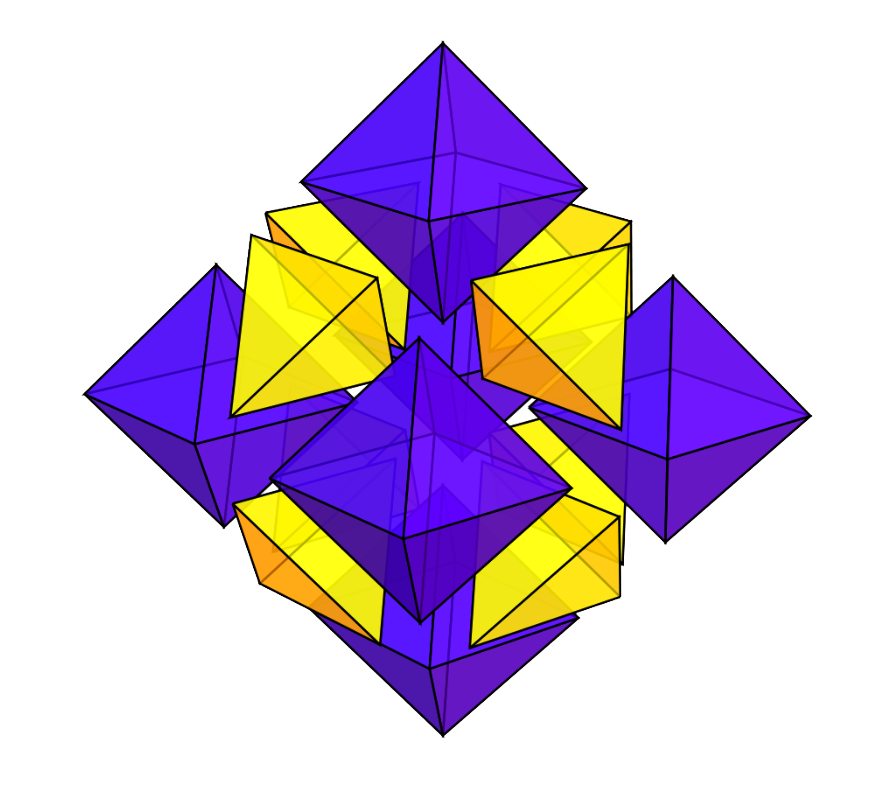
\includegraphics[height = 3.5cm]{./FigureLayout/tetra-exploded.PNG}
\end{center}


Right Part
\end{column}%
\end{columns}





	Delaunay -> Laguerre-Delaunay

	2d -> 3d

	\note{3d is very unintuitive. Number of neighors, angle relationships}




	Theoretical and practical
\end{frame}




\begin{frame}\frametitle{Laguerre-Delaunay}

\begin{itemize}
\item Generators are not points, but \alert{spheres}. 
\item $\gamma = \{p_1,\dots, p_n \} = \{(p'_1, p''_1), \dots , (p'_n, p''_n)\}$ can be thought of as \alert{marked point process}.
\item Metric is not Euclidean, but \alert{power distance}.
$$ d(q',p) = \|q'-p'\|^2 - p''^2$$
\end{itemize}



\definecolor{wrwrwr}{rgb}{0.3803921568627451,0.3803921568627451,0.3803921568627451}

\resizebox{0.7\textwidth}{!}{
	\begin{tikzpicture}[line cap=round,line join=round,>=triangle 45,x=1cm,y=1cm]
\clip(-34.06221132360224,19.559143724639345) rectangle (-8.217986359569402,34.582776229682544);
\draw [line width=4pt,color=wrwrwr] (-22.818487068133912,26.001637556556815) circle (5.131318559036773cm);
\draw [line width=4pt,color=wrwrwr] (-22.15663388793076,31.090093169232418)-- (-15.018487068133922,30.161637556556805);
\draw [line width=4pt,color=wrwrwr] (-22.818487068133912,26.001637556556815)-- (-22.15663388793076,31.090093169232418);
\draw [line width=4pt,color=wrwrwr] (-22.818487068133912,26.001637556556815)-- (-15.018487068133922,30.161637556556805);
\draw (-23.57696780445743,29.46311574805324) node[anchor=north west] {\Huge$p''$};
\draw (-19.93284265814484,32.36947322670743) node[anchor=north west] {\Huge$\sqrt{d(q',p)}$};
\draw (-14.567259620629372,30.804511507432096) node[anchor=north west] {\Huge$q'$};
\draw (-23.800533764353904,26.08726975361645) node[anchor=north west] {\Huge$p'$};
\draw (0.009240964620983672,0.35482776953204165) node[anchor=north west] {\Huge$p'$};
\draw (0.009240964620983672,0.35482776953204165) node[anchor=north west] {\Huge$p'$};
\draw (0.009240964620983672,0.35482776953204165) node[anchor=north west] {\Huge$p''$};
\begin{scriptsize}
\draw [fill=wrwrwr] (-22.818487068133912,26.001637556556815) circle (2.5pt);
\draw [fill=wrwrwr] (-15.018487068133922,30.161637556556805) circle (2.5pt);
\draw [fill=wrwrwr] (-22.15663388793076,31.090093169232418) circle (2pt);
\end{scriptsize}
\end{tikzpicture}
}

\end{frame}




\begin{frame}\frametitle{Theoretical}
	Based on [Dereudre et al. 2012 ] 

	Understand them as hypergraphs


	Provides very general conditions for existence
	BUT - not Laguerre, not MPP

	First step - rephrase it to MPP
\end{frame}






\begin{frame}\frametitle{Range condition}

	Best would be finite range, but we don't have that.



\begin{definition}
	A set $\Delta \in \mathcal B_0$ is a \textit{finite horizon} for the pair $(\eta,\x) \in \mathcal E$ and the hyperedge potential $\varphi$ if for all $\tilde{\x} \in \mathbf N_{lf}, \tilde{\x} = \x$ on $\Delta\times S$ 
$$(\eta,\tilde{\x})\in\mathcal E \text{ and } \varphi(\eta,\tilde{\x}) = \varphi(\eta,\x). $$
The pair $(\mathcal E, \varphi)$ satisfies the \textit{finite-horizon property} if each $(\eta,\x)\in \mathcal E$ has a finite horizon.
\end{definition}

\begin{itemize}
	\item \textit{Range condition}. There exist constants $\ell_R,n_R \in \mathbb N$ and $\delta_R < \infty$ such that for all $(\eta,\x) \in \mathcal E$ there exists a finite horizon $\Delta$ satisfying: For every $x,y \in \Delta$ there exist $\ell$ open balls $B_1, \dots, B_\ell$ (with $\ell \leq \ell_R$) such that
	\begin{enumerate}[-]
		\item the set $\cup^\ell_{i=1} \bar B_i$ is connected and contains $x$ and $y$, and 
		\item for each $i$, either $\text{diam} B_i \leq \delta_R$ or $\# (\x \cap (B_i\times S)) \leq n_R$.
	\end{enumerate}
\end{itemize}
\end{frame}


\begin{frame}\frametitle{Apollonius problem}

\definecolor{aqaqaq}{rgb}{0.6274509803921569,0.6274509803921569,0.6274509803921569}

\resizebox{0.4\textwidth}{!}{
\begin{tikzpicture}[line cap=round,line join=round,>=triangle 45,x=1cm,y=1cm]
\clip(-0.3382769769074499,-0.28262781541960746) rectangle (5.515106366556936,4.296783859173118);
\draw [line width=0.8pt,color=aqaqaq] (0,4)-- (0,0);
\draw [line width=0.8pt,color=aqaqaq] (0.8660254037844386,3.5)-- (0.8660254037844386,0.5);
\draw [line width=0.8pt,color=aqaqaq] (1.7320508075688772,4)-- (1.7320508075688772,0);
\draw [line width=0.8pt,color=aqaqaq] (2.598076211353316,3.5)-- (2.598076211353316,0.5);
\draw [line width=0.8pt,color=aqaqaq] (3.4641016151377544,4)-- (3.4641016151377544,0);
\draw [line width=0.8pt,color=aqaqaq] (0,2)-- (3.4641016151377544,0);
\draw [line width=0.8pt,color=aqaqaq] (0,1)-- (1.7320508075688772,0);
\draw [line width=0.8pt,color=aqaqaq] (0,2)-- (3.4641016151377544,4);
\draw [line width=0.8pt,color=aqaqaq] (0,3)-- (1.7320508075688772,4);
\draw [line width=0.8pt,color=aqaqaq] (0,1)-- (5.196152422706632,4);
\draw [line width=0.8pt,color=aqaqaq] (0,0)-- (5.196152422706632,3);
\draw [line width=0.8pt,color=aqaqaq] (1.7320508075688772,0)-- (5.196152422706632,2);
\draw [line width=0.8pt,color=aqaqaq] (3.4641016151377544,4)-- (5.196152422706632,3);
\draw [line width=0.8pt,color=aqaqaq] (1.7320508075688772,4)-- (5.196152422706632,2);
\draw [line width=0.8pt,color=aqaqaq] (0,4)-- (5.196152422706632,1);
\draw [line width=0.8pt,color=aqaqaq] (0,3)-- (5.196152422706632,0);
\draw [line width=0.8pt,color=aqaqaq] (3.4641016151377544,0)-- (5.196152422706632,1);
\draw [line width=0.8pt,color=aqaqaq] (4.330127018922193,3.5)-- (4.330127018922193,0.5);
\draw [line width=0.8pt,color=aqaqaq] (5.196152422706632,4)-- (5.196152422706632,0);
\begin{scriptsize}
\draw [fill=aqaqaq] (0,0) circle (1.5pt);
\draw [fill=aqaqaq] (0,1) circle (1.5pt);
\draw [fill=aqaqaq] (0.8660254037844386,0.5) circle (1.5pt);
\draw [fill=aqaqaq] (0,2) circle (1.5pt);
\draw [fill=aqaqaq] (0,3) circle (1.5pt);
\draw [fill=aqaqaq] (0,4) circle (1.5pt);
\draw [fill=aqaqaq] (0.8660254037844386,1.5) circle (1.5pt);
\draw [fill=aqaqaq] (0.8660254037844386,2.5) circle (1.5pt);
\draw [fill=aqaqaq] (0.8660254037844386,3.5) circle (1.5pt);
\draw [fill=aqaqaq] (1.7320508075688772,4) circle (1.5pt);
\draw [fill=aqaqaq] (1.7320508075688772,3) circle (1.5pt);
\draw [fill=aqaqaq] (1.7320508075688772,2) circle (1.5pt);
\draw [fill=aqaqaq] (1.7320508075688772,1) circle (1.5pt);
\draw [fill=aqaqaq] (1.7320508075688772,0) circle (1.5pt);
\draw [fill=aqaqaq] (2.598076211353316,3.5) circle (1.5pt);
\draw [fill=aqaqaq] (2.598076211353316,2.5) circle (1.5pt);
\draw [fill=aqaqaq] (2.598076211353316,1.5) circle (1.5pt);
\draw [fill=aqaqaq] (2.598076211353316,0.5) circle (1.5pt);
\draw [fill=aqaqaq] (3.4641016151377544,4) circle (1.5pt);
\draw [fill=aqaqaq] (3.4641016151377544,3) circle (1.5pt);
\draw [fill=aqaqaq] (3.4641016151377544,2) circle (1.5pt);
\draw [fill=aqaqaq] (3.4641016151377544,1) circle (1.5pt);
\draw [fill=aqaqaq] (3.4641016151377544,0) circle (1.5pt);
\draw [fill=aqaqaq] (4.330127018922193,3.5) circle (1.5pt);
\draw [fill=aqaqaq] (4.330127018922193,2.5) circle (1.5pt);
\draw [fill=aqaqaq] (4.330127018922193,1.5) circle (1.5pt);
\draw [fill=aqaqaq] (4.330127018922193,0.5) circle (1.5pt);
\draw [fill=aqaqaq] (5.196152422706632,4) circle (1.5pt);
\draw [fill=aqaqaq] (5.196152422706632,3) circle (1.5pt);
\draw [fill=aqaqaq] (5.196152422706632,2) circle (1.5pt);
\draw [fill=aqaqaq] (5.196152422706632,1) circle (1.5pt);
\draw [fill=aqaqaq] (5.196152422706632,0) circle (1.5pt);
\end{scriptsize}
\end{tikzpicture}
}

\end{frame}



\begin{frame}\frametitle{Practical}
	\framesubtitle{Implementation}

	3D much more difficult

	Need to recalculate tessellation each step

	Decided to write own, more general in C++

	Failed, went to CGAL

	MCMC MH 

	Additional analysis done in Python and Mathematica

\begin{center}
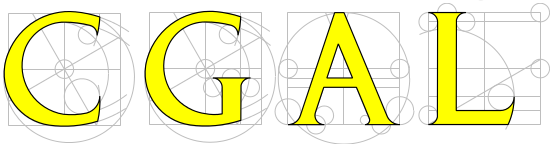
\includegraphics[height = 1cm]{./FigureLayout/cgal.png}
\end{center}

https://github.com/DahnJ/General-Increment-Decrement.git

https://github.com/DahnJ/Gibbs-Laguerre-Delaunay.git

% Available on github
	
\end{frame}






\begin{frame}\frametitle{Practical}
	Some results, e.g. role of theta (+reduction to PPP)
	
\end{frame}


\begin{frame}[noframenumbering]\frametitle{Summary and references, I guess?}
	
D. Dereudre and F. Lavancier. Practical simulation and estimation for
Gibbs Delaunay-Voronoi tessellations with geometric hardcore interaction.
Computational Statistics and Data Analysis, 55(1):498-519, 2011.

D. Dereudre, R. Drouilhet, and H.O. Georgii. Existence of gibbsian point
processes with geometry-dependent interactions. Probability Theory and
Related Fields, 153(3):643-670, 2012


Fropuff. The vertex configuration of a tetrahedral-octahedral honeycomb., 2006.
URL https://en.wikipedia.org/wiki/File:TetraOctaHoneycomb-VertexConfig.svg

\end{frame}



%  \section{Simulation and Estimation}
%  \framesection{}
%  
%  
%  \begin{frame}\frametitle{Two-step procedure}
%  \begin{small}
%  We have $4$ parameters to estimate
%  \begin{itemize}
%  \item Hard-core parameters.
%      \begin{itemize}
%      \item The minimum face area $\epsilon$,
%      \item the maximum circumradius $\alpha$.
%      \end{itemize}
%  \item Smooth parameters.
%      \begin{itemize}
%      \item The multiplier of $Sur(T)$, $\theta$,
%      \item the intensity of the underlying Poisson point process, $z$.
%      \end{itemize}
%  \end{itemize}
%  \vspace{5mm}
%  This is done through a \alert{two-step procedure}
%  \begin{enumerate}
%      \item Estimate the hardcore parameters $(\epsilon, \alpha)$ directly.
%      \item Estimate the smooth parameters $(\theta,z)$ by \alert{Maximum Pseudo-Likelihood Estimation} (MPLE) using the estimates $(\hat\epsilon,\hat\alpha)$.
%  \end{enumerate}
%  \end{small}
%  
%  
%  \end{frame}
%  
%  \begin{frame}\frametitle{Two-step procedure}\framesubtitle{1. Hardcore interaction parameters estimation}
%  \begin{small}
%  [Dereudre, Lavancier (2009)] only proves consistence for a single parameter (although experimentally both work).\newline
%  
%  Thanks to the fact that the hardcore parameter $\alpha$ satisfies
%  $$ \text{if } \alpha < \alpha' \text{ then  } \forall \Lambda, \; H^{\epsilon,\alpha,\theta}_\Lambda(\gamma) < \infty \Rightarrow  H^{\epsilon,\alpha',\theta}_\Lambda(\gamma)<\infty,$$ 
%  its consistent estimator is
%  $$\hat\alpha = \inf\{\alpha > 0, H_\Lambda(\gamma) < \infty \},$$
%  which in practice is estimated as
%  $$\hat\alpha = \max\{r(T), T\in \mathcal LDel_\Lambda(\gamma)\}.$$
%  
%  The estimate $\hat\alpha$ is then used in the pseudo-likelihood function in the second estimation step.
%  
%  \end{small}
%  \end{frame}
%  
%  
%  %%%%% Slide
%  % ----------------------------------------------------------------------------------------
%  \begin{frame}\frametitle{Two-step procedure}\framesubtitle{2. Maximum pseudolikelihood}
%  MPLE depends on GNZ, which works only for \alert{hereditary} energy functions.
%  $$H(\gamma) < \infty \Rightarrow H(\gamma \setminus \{x\}) < \infty \quad x \in \gamma$$
%  
%  \begin{center}
%  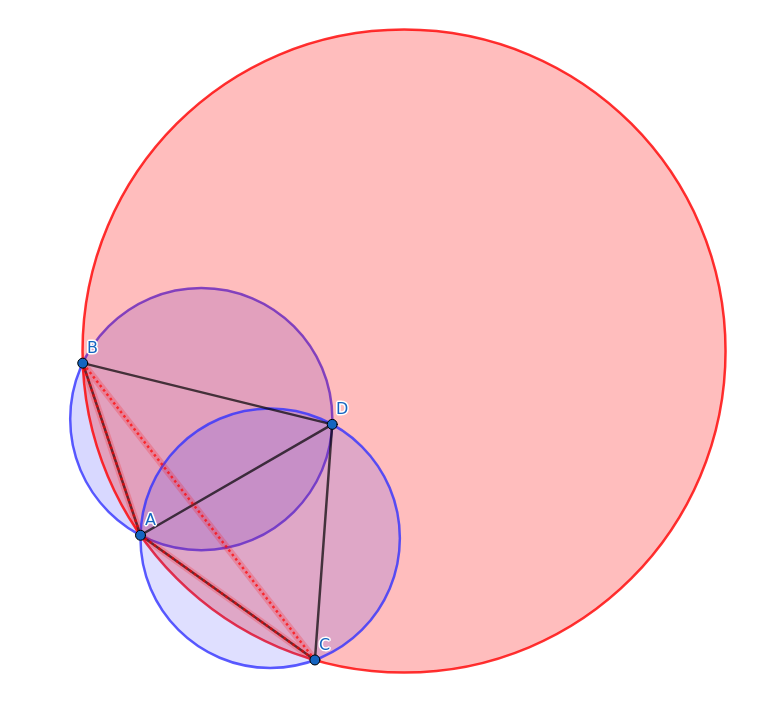
\includegraphics[height = 3.5cm]{./FigureLayout/hereditarity.png}
%  \end{center}
%  \pause
%  However [Dereudre, Lavancier (2009)] proved that GNZ still holds if we restrict ourselves to \alert{removable points}.\newline
%  
%  We say a point $x\in \gamma$ is removable if $H(\gamma \setminus \{x\}) < \infty$. Denote $\alert {\mathcal R^\alpha(\gamma)}$ the set of removable points in $\gamma$. 
%  
%  
%  \end{frame}
%  
%  %%%%% Slide
%  % ----------------------------------------------------------------------------------------
%  \begin{frame}\frametitle{Two-step procedure}\framesubtitle{2. Maximum pseudolikelihood}
%  \begin{small}
%  The pseudolikelihood function is
%  $$ PLL_{\Lambda_W}(\gamma,z,\alpha, \theta) = \int_{\Lambda_W } z \exp (-h^{\alpha,\theta}(x,\gamma)) dx + \sum_{x\in\mathcal R^\alpha(\gamma)\cap \Lambda_W } \big(h^{\alpha,\theta}(x,\gamma\setminus\{x\}) - \ln(z)\big),
%  $$
%  
%  
%  The estimates $\hat\theta$ and $\hat z$ are obtained through minimizing the $PLL_{\Lambda_W }$ function. 
%  $$(\hat z, \hat\theta) = \text{argmin}_{z,\theta} PLL_{\Lambda_W } (\gamma, z, \hat\alpha,\theta).$$
%  
%  \pause
%  Differentiation yields the estimate $\hat z$ 
%  
%  $$\hat z = \frac{\mbox{card}(\mathcal R^{\hat\alpha}(\gamma)\cap \Lambda_W)}{\int_{\Lambda_W} \exp{\left( -h^{\hat\alpha,\theta}(x,\gamma)\right)} dx},$$
%  \pause
%  and the estimate $\hat\theta$ as the solution of
%  
%  $$z \int_{\Lambda_W} (h^{\hat\alpha,1}(x,\gamma)\exp{\left(-h^{\hat\alpha,\theta}(x,\gamma)\right)}) dx = \sum_{x \in \mathcal R^{\hat\alpha}(\gamma)\cap \Lambda_W} h^{\hat\alpha,1}(x,\gamma\setminus\{x\}).$$
%  
%  \end{small}
%  \end{frame}
%  
%  
%  
%  \begin{frame}\frametitle{Two-step procedure}\framesubtitle{2. Maximum pseudolikelihood - practical implementation}
%  \begin{small}
%  
%  To obtain the estimate for $\theta$, substitute the expression for $\hat z$ into the equation for $\theta$.
%  \begin{equation}\label{eq}
%  \frac{\int_{\Lambda_W } (h^{\hat\alpha,1}(x,\gamma)\exp{\left(-h^{\hat\alpha,\theta}(x,\gamma)\right)}) dx} {  \int_{\Lambda_W } \exp{\left( -h^{\hat\alpha,\theta}(x,\gamma)\right)} dx} 
%  = \frac {\sum_{x \in \mathcal R^{\hat\alpha}(\gamma)\cap \Lambda_W } h^{\hat\alpha,1}(x,\gamma\setminus\{x\})} { \mbox{card}(\mathcal R^\alpha(\gamma)\cap \Lambda_W ) }. 
%  \end{equation}
%  After some algebraic manipulation, we obtain the equation
%  
%  $$\int_{\Lambda_W} \exp{\left(-\theta h^{\hat\alpha, 1}(x,\gamma)\right)} (h^{\hat\alpha, 1}(x,\gamma) - c) dx = 0 ,$$
%  
%  where $c$ is the RHS of (\ref{eq}), which is independent of $\theta$. \newline
%  
%  After $\hat\theta$ is estimated, we then obtain the estimate $\hat z$ using the esitmate $\hat\theta$ instead of $\theta$.
%  
%  All integrals are estimated by MC-integration.
%  \end{small}
%  \end{frame}
%  
%  
%  \begin{frame}\frametitle{Estimation results}
%  
%  
%  \end{frame}






\begin{frame}[noframenumbering]\frametitle{(1) (Reinforced) general position}

\begin{definition}
Let $\x \in \mathbf N_{lf}$. We say $\x$ is in \textbf{general position} if 
$$ \eta \subset \x, 2 \leq \mathrm{card}(\eta) \leq 4 \Rightarrow \eta' \text{ is affinely independent in } \mathbb R^3. $$   
Denote $\mathbf N_{gp}\subset \mathbf N_{lf}$ the set of all locally finite configurations in general position.
\end{definition}
We call points $\{x'_0,x'_1,\dots,x'_k\}\subset \mathbb R^3,k \in \mathbb N$ \textit{cospherical} if there exists a sphere $S\subset \mathbb R^3$ such that $\{x'_0,\dots, x'_k\} \subset S$. In this text, a sphere will always refer to the boundary of a ball, never to the interior.

\begin{definition}
Let $\x \in \mathbf N_{gp}$. We say $\x$ is in \textbf{reinforced general position} if 
$$ \eta \subset \x, \mathrm{card}(\eta) = 4 \Rightarrow \eta' \text{ is not cospherical.} $$   
Denote $\mathbf N_{rgp}$ the set of all locally finite configurations in reinforced general position.
\end{definition}

\end{frame}



\begin{frame}[noframenumbering]\frametitle{(2) Set $\mathcal E_\Lambda$}

$$\mathbf N_\Lambda = \{ \nu \in \mathbf N_{lf}: \nu( (\mathbb R^3 \setminus \Lambda) \times S) = 0 \}$$



\begin{definition}\label{def:Eset} Let $\Lambda \in \mathcal B_0$. Define the set 
	$$\mathcal E_\Lambda(\x) := \{ \eta \in \mathcal E(\x): \varphi(\eta,\zeta \cup \x_{\Lambda^c}) \neq \varphi(\eta,\x) \text{ for some } \zeta \in \mathbf N_\Lambda \}.$$
\end{definition}

Recall that we have defined $\varphi=0$ on $\mathcal E^c$. This means that for $\eta \in \mathcal E(\x)$ such that $\varphi(\eta,\x)\neq 0$ we have
$$\eta \notin \mathcal E(\zeta \cup \x_{\Lambda^c})\text{ for some }\zeta \in \mathbf N_{\Lambda} \Rightarrow \eta \in \mathcal E_{\Lambda}(\x).$$ 

\end{frame}



\begin{frame}[noframenumbering]\frametitle{(3) Characterization of sets $\mathcal D_\Lambda$ and $\mathcal {LD}_\Lambda$}


The condition in the definition can also be equivalently stated as 
\begin{equation}\label{eq:equivregular}\text{There is no point } q\in\x \text{ such that } d(p'_\eta,q)<p''_\eta.\end{equation}

[$\mathcal E_\Lambda(\x)$ for $\mathcal D$ and $\mathcal {LD}$] 
	For $\mathcal D$, we have that 
	$$\eta \in \mathcal D_\Lambda(\x)\iff B(\eta) \cap \Lambda \neq \emptyset.$$ 
	For $\mathcal {LD}$, using the characterization \eqref{eq:equivregular}, we obtain 
	$$\eta \in \mathcal {LD}_\Lambda(\x) \iff d(p'_\eta;\Lambda) < \sqrt{p''_\eta + W},$$
	where $d(p'_\eta;\Lambda) = \inf\{\|p'_\eta - x\|: x \in \Lambda\}$ is the distance of $p'_\eta$ from $\Lambda$.    


\end{frame}




\end{document}
